\section{Sensordaten aus Simulator CoppeliaSim}
Insgesamt wurden vier Routen über 20 Zyklen jeweils zweimal erfasst.
Das geschah einmal für Trainingsdaten und einmal für Testdaten, wobei die letzten fünf Zyklen der
Trainingsdaten als Validationsmenge genutzt werden.
Dabei wurden alle 50ms die xyz-Koordinaten, Accelerometerdaten und Gyroskopdaten erfasst, sowie Lichtintensität und Metadaten.
Zu den Metadaten gehören Zeitstempel, Beschriftung des Routenabschnitts und Beschriftung des derzeitigen Zykluses.
Ein Zyklus ist der vollständige Umlauf einer Route.
\newline
\newline
Abbildung \ref{fig:simple_square_labeled} zeigt eine der vier Routen \glqq simple\_square\grqq.
Jede Route ist mit Markierungen für Zyklen und Standorte ausgestattet.
Die Zyklusmarkierung wird genutzt, um die Datensätze mit dem derzeitigen Zyklus zu beschriften.
Jedes Mal, wenn die Sensorenbox diese Markierung überschreitet, wird der Zähler für den Zyklus inkrementiert.
\newpage
Die Standortmarkierung wird genutzt, um die Datensätze mit dem derzeitigen Routenabschnitt zu beschriften.
Jedes Mal, wenn die Sensorenbox diese Markierung überschreitet, wird der derzeitige Wert für den Routenabschnitt auf den Wert der Markierung gesetzt.
Dabei werden alle aufgenommenen Datensätze immer mit dem derzeitigen Wert für den Routenabschnitt annotiert.
\begin{figure}[h!]
    \centering
    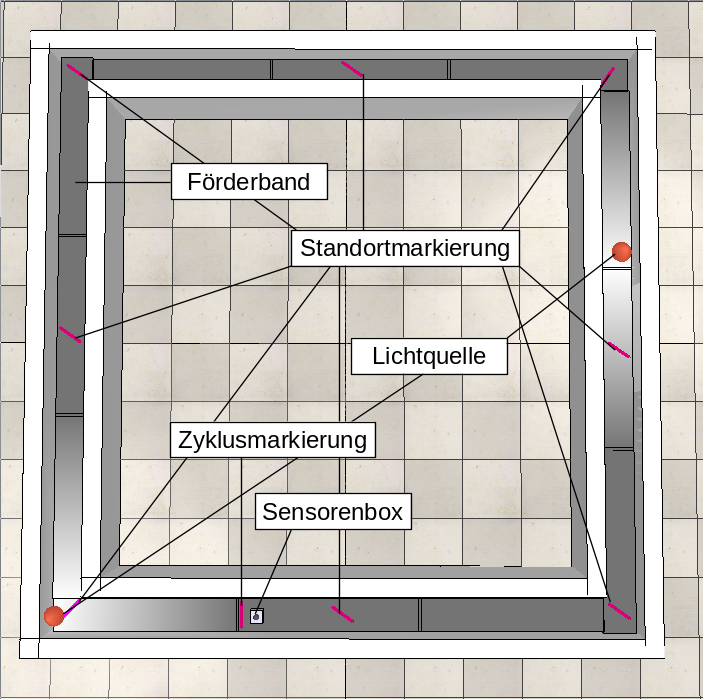
\includegraphics[width=0.75\linewidth]{images/simple_square_labeled.png}
    \caption{Modell der Route \glqq simple\_square\grqq\ in CoppeliaSim mit Beschriftungen.}
    \label{fig:simple_square_labeled}
\end{figure}
\newline
\newline
Neben \glqq simple\_square \grqq\ gibt es noch drei weitere Routen (siehe Abbildungen \ref{fig:long_rectangle}, \ref{fig:rectangle_with_ramp} und \ref{fig:many_corners}).
Die Route \glqq long\_rectangle\grqq\ weist lange Pfade mit wenig Änderungen auf.
Die Route \glqq rectangle\_with\_ramp\grqq\ besitzt zusätzlich zwei Rampen, wodurch Höhenunterschiede simuliert werden.
Die Route \glqq many\_corners\grqq\ ist sehr komplex und hat viele verschiedene Standorte.
Die Förderbänder können verschiedene Geschwindigkeiten haben mit sowohl abrupten Übergängen als auch fließenden Übergängen zueinander.
\newline
\newline
Je nach Kodierungsart (siehe Kapitel \ref{sec:model_location_encoding}) müssen die Knoten und Kanten des zyklischen Graphen als Standorte kodiert werden.
Mian hatte in seiner Arbeit die Kanten während der simulation markiert \cite{naveedThesis}.
In dieser Arbeit wurde der Programm-Code seiner Arbeit für die Simulation übernommen, weswegen die aufgenommen Daten initial genau so beschriftet sind.
Aus diesem Grund müssen die aufgenommen Datensätze transformiert werden, sodass nicht die Kanten, sondern entweder Knoten oder Knoten und Kanten kodiert werden.
Zu einem Knoten gehören die Datensätze, die sich in einem Umkreis vom ersten Datensatz befindet, der eine einzigartige Beschriftung in der Simulation erhalten hatte.
Bei dem Kodierungsansatz, der nur die Knoten kodiert, werden die restlichen Datensätze als \textit{unbekannt} beschriftet.
Bei dem Kodierungsansatz, der Knoten und Kanten kodiert, werden die restlichen Datensätze mit einer neuen einzigartigen Beschriftung markiert, die abhängig von der
topologischen Position der zuvor bestimmten Knoten ist.
